\subsubsection{Functional Requirements}
\begin{itemize}
  \item The user has to provide her credentials. 
  \item The user has to provide her payment information.
  \item The system shall give back a password that can be used for log-in.
\end{itemize}


\subsubsection{Scenario 1}
Mark has been told that a new awesome car-sharing service just launched, he then decide to download the mobile application and register as a new user. After filling the sign-up module a confirmation e-mail is sent to Mark containing his new credentials.


\subsubsection{Scenario 2}
Susan was browsing the net when an advertisement caught her attention, it says: "PowerEnJoy is the new planet-friendly car sharing service! Register now and get a discount on your first ride!". She then clicks the advertisement and opens the web application: the first page is a Sign-up page and Susan fills up her personal informations and confirms. Unfortunately the informations provided are not complete and the system signals an error, she notices that the driving licence's informations are missing and compiles the remaining part of the module before submitting it and receiving a confirmation e-mail.


\subsubsection{Mockups}
\begin{figure}[!ht]
  \centering
  \vspace{0.2cm}
  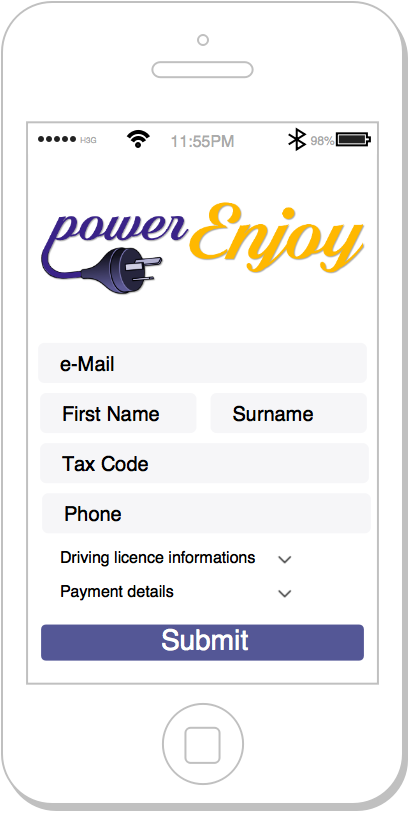
\includegraphics[width=0.25\textwidth]{/RASD/System_Functions/registration_mockup}\\
  \vspace{0.4cm}
  %\caption{Mockup for the registration mobile page} 
  \label{fig:registration_mockup} 
\end{figure}
% maybe home page mockup here 


\subsubsection{Use-case table}
\begin{center}
  \begin{tabular}{ l | p{10cm} }
    \hline
    Actors & Guest\\ \hline
    Goal & G\ref{itm:goal-registration}\\ \hline
    Entry conditions & The Guest enters the Sign-up page in the web/mobile application. 
     \\ \hline
    Flow of events &
    \begin{itemize} % todo: shrink items
      \item The Guest is shown a form to fill with her personal informations (e-mail, name, surname, tax code, phone number, driving license, payment information) %da scegliere se l'ID viene scelto dal system o dal Guest 
      \item The Guest fills the form and confirm the provided information.
      \item The system sends a confirmation e-mail to the Guest's personal e-mail with an activation link.
      \item The Guest clicks the link in the system's e-mail.
      \item The system allocates the User in the database.
      \item The system sends an e-mail to the User's e-mail with her personal \gls{pwd}.
      \item The system loads the User's homepage.
    \end{itemize} \\ \hline
    Exit conditions & The Guest is registered to PowerEnJoy and became an User. Now the User is in her homepage. \\ \hline
  	Exceptions & 
    \begin{itemize}
      \item The Guest provides an e-mail or a phone number or a tax code already used (in this case the system signals an error).
      \item The Guest does not fill one or more fields in a form (in this cases the system does not allow to proceed and signals an InformationLack).
      \item The Guest provided wrong payment information (in this case the system signals an error).
      \item The Guest provided wrong drive license information (in this case the system signals an error).
      \item The system is not able to complete the operation due to some internal issues or connection broken (the system signals a ConnectionFailure). % modifiable exceptions names
    \end{itemize} \\ \hline
  \end{tabular}
\end{center}


\subsubsection{Sequence diagram}
\begin{figure}[!ht]
  \centering
  \vspace{0.2cm}
  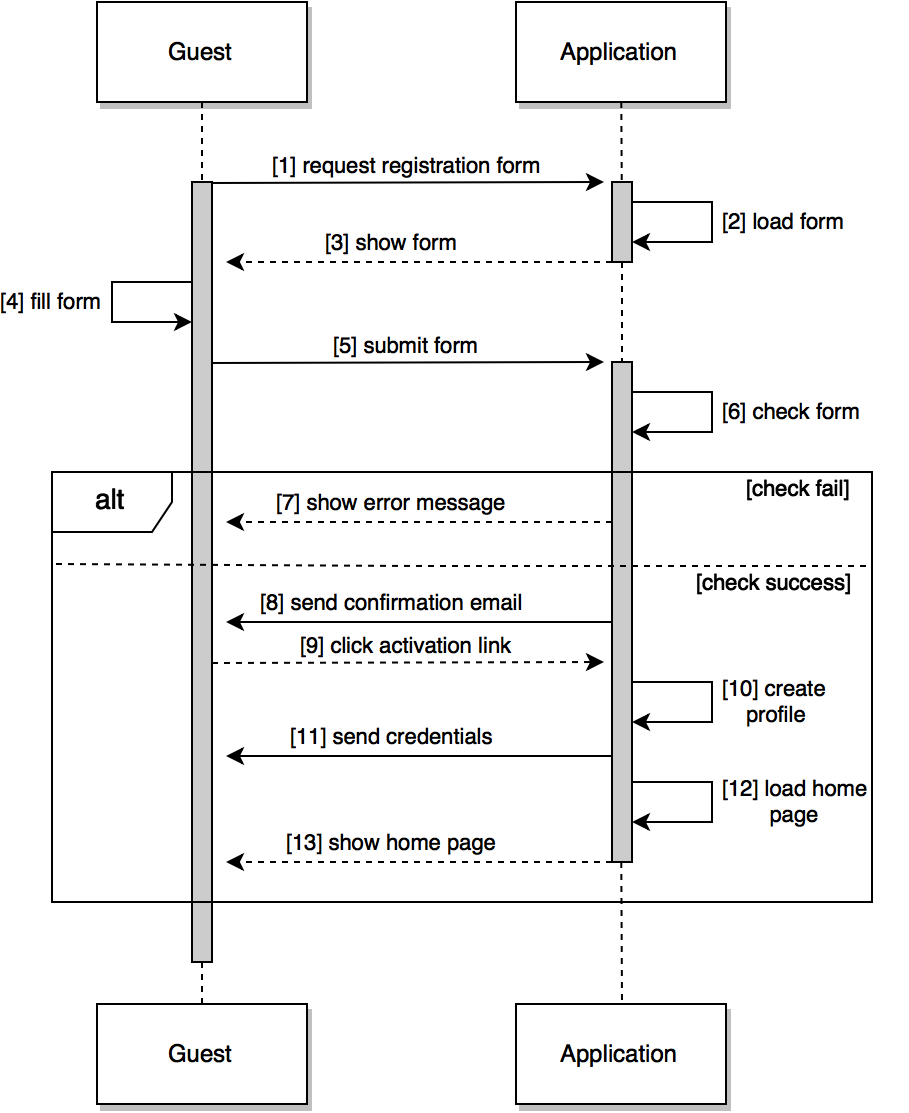
\includegraphics[width=0.6\textwidth]{/RASD/System_Functions/registration_sequence}\\
  \vspace{0.4cm}
  %\caption{Sequence diagram for the registration procedure} 
  \label{fig:registration_sequence} 
\end{figure}
